\documentclass[a4paper,11pt]{article}
\usepackage[a4paper,margin=1in,footskip=0.25in]{geometry}
\usepackage[utf8]{inputenc}

% science
\usepackage{amsmath}
\usepackage{array}
\usepackage{siunitx}

% code
% Default fixed font does not support bold face
\DeclareFixedFont{\ttb}{T1}{txtt}{bx}{n}{10} % for bold
\DeclareFixedFont{\ttm}{T1}{txtt}{m}{n}{10}  % for normal

% Custom colors
\usepackage{color}
\definecolor{deepblue}{rgb}{0,0,0.5}
\definecolor{deepred}{rgb}{0.6,0,0}
\definecolor{deepgreen}{rgb}{0,0.5,0}

\usepackage{listings}

% Python style for highlighting
\newcommand\pythonstyle{\lstset{
        language=Python,
        basicstyle=\ttm,
        morekeywords={self},              % Add keywords here
        keywordstyle=\ttb\color{deepblue},
        emph={MyClass,__init__},          % Custom highlighting
        emphstyle=\ttb\color{deepred},    % Custom highlighting style
        stringstyle=\color{deepgreen},
        frame=tb,                         % Any extra options here
        showstringspaces=false
}}


% Python environment
\lstnewenvironment{python}[1][]
{
    \pythonstyle
    \lstset{#1}
}
{}

% Python for external files
\newcommand\pythonexternal[2][]{{
        \pythonstyle
        \lstinputlisting[#1]{#2}}}

% Python for inline
\newcommand\pythoninline[1]{{\pythonstyle\lstinline!#1!}}

% layout
\usepackage{float}
\usepackage{parskip}
\usepackage{graphicx}
\usepackage{circuitikz}
\usepackage{longtable}
\usepackage{hyperref}
\usepackage[export]{adjustbox}
\usepackage{hhline}

% referencing
\usepackage[style=apa]{biblatex}
\addbibresource{ratio.bib}
\usepackage{hyperref}

% table centering
\renewcommand{\arraystretch}{1.3}
\newcolumntype{P}[1]{>{\raggedright\arraybackslash}p{#1}}
\newcommand{\tptt}{$\times\,$}

% figures labelings
\usepackage{chngcntr}
\counterwithin{figure}{section}

\usepackage{caption}
\usepackage{subcaption}
\usepackage{wrapfig}

\title{Estimating the quality of YouTube videos based on its likes and dislikes}

\author{}
\date{\vspace{-8ex}}

\begin{document}

% Planning
% Introduction
% Definition
% Steps of exploration
% Simulation Approach
% Statistical Approach
% Bayensian Approach
% Conclusion




\maketitle

\section{Introduction}

\begin{wrapfigure}{r}{0.45\textwidth}
    \centering
    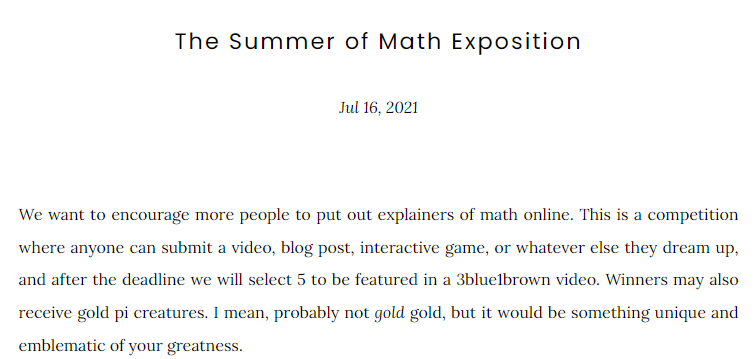
\includegraphics[width=0.5\textwidth]{assets/som1.png}
    \caption{The SoME1 event}
    \label{fig:some1}
\end{wrapfigure}

The topic of my exploration originates from a personal need I've developed in the school holidays.

I am familiar with the maths channel 3Blue1Brown (3B1B) on YouTube through a self learning playlist on the topic of linear algebra in year 1 IB, and was patiently waiting for a new video for it is the holidays. When Grant (owner of 3B1B) announced a contest (figure \ref{fig:some1}) not long after encouraging amateur video makers to share their hidden maths knowledges, I was understandably very excited to have my entire YouTube home page filled with the new maths videos. While I did find some brilliantly made videos like ``\href{https://www.youtube.com/watch?v=aVwxzDHniEw}{The Beauty of B\'{e}zier Curves}'' by Freya Holm\'{e}r, and an explanation of ``\href{https://www.youtube.com/watch?v=78wz4KSzUvo}{Noether's Theorem}'' by Orla M, I quickly realized my inability to view all of the thousands of videos within a two week holiday. The solution? I will only watch the best ones.

But how do you tell if a YouTube video is the ``best'' out of the bunch? Visual indicators like interesting thumbnails may be attempting, but one should really not judge the book by its cover; while comparing view counts is fast, it is against the purpose of the maths event --- to discover new talented video creators. So I am left with the only other numerical indicators, to judge the quality of the video through the amount of likes and dislikes it has. While this measure have its limitations: the internet audience is biased in political and social values, it is certainty the most interesting metric.

%(At the time of writing, the company YouTube has removed the dislike count on all videos, which is disappointing)

Therefore within this exploration, I will be finding an equation relating the amount of likes and dislikes a YouTube video has to the best estimate of its perceived quality by the viewers. I will be using multiple methods such as simulations, statistical distributions, and a Bayesian approach to deduce the relationships between the two variables. It will be crucial that I evaluate the pros and cons of each approach, both in its solution but also in its derivation, and use my knowledge to rank five videos from the SoME1 event (table \ref{tbl:videos}, appendix).
%\begin{wrapfigure}{r}{0.4\textwidth}
%    \centering
%    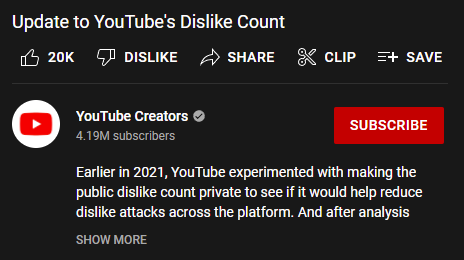
\includegraphics[width=0.45\textwidth]{assets/intro.png}
%    \caption{Hidden Dislikes}
%    \label{fig:hidden}
%\end{wrapfigure}

%This topic is chosen out of my curiously towards a very insignificant change. For I often procrastinate when doing my homework, I stumbled across a post on an online forum announcing the the popular internet video sharing platform of YouTube of removing their dislike counts (shown in Figure \ref{fig:hidden}). As usual, I dug into the comment section of the announcement and saw all the various complaints that one will expect on the internet, all but one has caught my eye:

%\begin{quote}
%    Dislike counts were necessary to spot clickbait, scams, fake tutorials, blatant misinformation, etc. --- Element 115 (internet user)
%\end{quote}

%The usage of likes and dislikes as a metric of legibility and quality is something that I knew and used extensively, mostly in saving my precious time in judging the qualities of the a series of maths videos made for the trend ``Summer of Math Exposition'' (SoME1) consisting of mostly amateur video makers. While the removal of the dislike counts demonstrated on how reliant I was on a simple number, it also led me to wonder of my technique in judging the quality of a video, especially in the SoME1 series for the like and dislike counts are often low. Therefore I felt this topic is worth exploring for its practicality.

% aim here

% 5 videos
% https://www.youtube.com/watch?v=-LVhZtFwZzM
% 705 2
% https://www.youtube.com/watch?v=E9IQY8LzzO8
% 35 5
% https://www.youtube.com/watch?v=vc_-aCeP7y8
% 25 0
% https://www.youtube.com/watch?v=tc53eCUvJyY
% 15 0 756
% https://www.youtube.com/watch?v=TJyCbR29Mds
% 4 0 138

\begin{figure}[H]
    \centering
    \begin{tabular}{c|c|c|c|c|c}
        & Video A & Video B & Video C & Video D & Video E \\
        \hline
        \hline
        Views & 138 & 440 & 467 & 756 & 10907 \\
        \hline
        Likes & 4 & 25 & 34 & 15 & 705 \\
        \hline
        Dislikes & 0 & 0 & 5 & 0 & 2
    \end{tabular}
    \captionof{table}{}
    \label{tbl:videos}
\end{figure}


\section{Keywords}

First we have to define some keywords which are used from this point onward. All YouTube videos are referred to as videos; the \textbf{ratings} of a video are its likes and dislikes, which are both positive integers; the \textbf{likeability} is the metric used to convey the quality of a video, and is defined as a probability between 0 and 1, representing the mean probability of a viewer rating the video to select ``like''. (For example, a likeability of $0.5$ means that on average, a person rating the video is pressing the like button 50\% of the time) The focus would be to find a mathematical definition of this likeability.

To showcase an initial attempt at defining this value, consider the two following videos:

% the two videos
\begin{figure}[H]
    \centering
    
\includegraphics[width=0.7\textwidth]{assets/s_vid2.png}
    \caption{Video one}
    \label{fig:vid1}
\end{figure}

\begin{figure}[H]
    \centering
    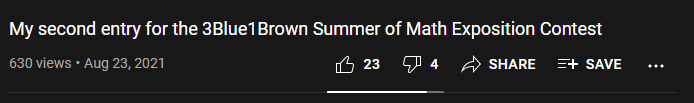
\includegraphics[width=0.7\textwidth]{assets/s_vid1.png}
    \caption{Video two}
    \label{fig:vid2}
\end{figure}

Figure \ref{fig:vid1} is a video with 6 likes and 1 dislike. Figure \ref{fig:vid2} is a video with 23 likes and 4 dislikes. Naively, it is tempting to calculate the likeabilities ($L_n$) of the two videos by dividing the amount of likes ($x$) against the total amount of ratings ($n$). This will be called as the \textbf{naive likeability}, and is defined by:

\[
L_n = \frac{x}{n}.
\]

The naive likeabilities of video one ($L_1$) and video two ($L_2$) are thus as follow:
\begin{align*}
    L_{1} &= \frac{6}{6+1} \approx 0.857, \,\, L_{2} = \frac{23}{23 + 4} \approx 0.851.
\end{align*}

If we assume this naive mathematical definition of the likeabilities represents our language definition, then we can rate the first video higher than the second because it has a higher likeability ($0.857 > 0.851$). So we should watch video one first, right?

However, the calculations are unlikely to match our proper definitions of likeability, simply because they failed to take the total amount of ratings into consideration. While video one has a higher like to dislike ratio than video two, there are fundamentally less overall ratings available. Thus our method also needs to factor in the amount of information we can see, to include a factor of certainty, almost.

This can be illustrated with an example taken to the extreme. A video with only one like and zero dislikes have a naive likeability of 100\%, but can we really be sure that it is of a higher quality than a video with 1000 likes and 1 dislike (naive likeability of 99.9\%)?

Therefore the naive likeability definition is uninclusive of all information but is fast. Nevertheless, table \ref{tbl:naive} shows the five videos as ranked by their naive likeabilities.

\begin{figure}[H]
    \centering
    \begin{tabular}{c|c|c|c|c|c}
        & Video A & Video B & Video C & Video D & Video E \\
        \hline
        \hline
        Naive Likeability & 1.000 & 1.000 & 0.872 & 1.000 & 0.997
    \end{tabular}
    \captionof{table}{}
    \label{tbl:naive}
\end{figure}


\section{Simulation}
For any statistical or probabilistic question, it is always helpful to start with a simulation of some kind. This is because a simulation allows me to both describe the problem as well as to approach a numerical solution, guaranteed by the law of large numbers --- stating that the statistical descriptions of a sample will tend towards that of the true descriptions as sample size increases.

% description of what I did
To do this, I've used Python 3.7 to write a small piece of code that does the calculations, and used a Python library called Matplotlib to graph the numbers.

Using video one (6 likes and 1 dislike) as an example, notice that it is theoretically possible for the video likeability to be of any probability except 0 and 1, for there is still a non-zero probability of receiving 6 likes on a video with 1\% likability, albeit very unlikely. Therefore I thought to define the likeability of a video by the average of all the possible likeabilities weighted by how likely they are to occur, as it matches our literal definition of ``the mean probability of a viewer rating the video to select like''.

The pseudocode for our simulation will look as follow:

\begin{python}
1   weighted = 0
2   for likeability in 0..1:
3       occurrence = simulate_occurence(likeability)
4
5       weighted += likeability * occurence / sample_size
6       plot(likeability, occurence)
\end{python}

The breakdown of this piece of code is as follows:

I first defined a variable \pythoninline{weighted} to hold the weighted average of the likeabilties:

\begin{python}
1   weighted = 0
\end{python}

Then I loop over all possible likeabilities from 0 to 1 using a \textit{for in} loop:
\begin{python}
2   for likeability in 0..1:
\end{python}

For each likability, I considered a simulation of 1000 times a group of 7 people rating the video. This is performed in the function \pythoninline{simulate_occurence}(appendix), which takes the likeability as an input. It outputs the \# of times the ratings by those 7 people matches the 6 likes and 1 dislike of video one, and saves this in the variable called \pythoninline{occurrence}.

\begin{python}
3       occurrence = simulate_occurence(likability)
\end{python}

To calculate the weighted averages (statistical mean) of the likeability, I've used the discrete mean formula, which states the mean ($\mu$) is the sum of the likeabilities ($L_i$) multiplied by their respective probabilities ($f(L_i)$):
\[
    \mu = \sum_{i = 1}^{n} L_i f(L_i)
\]

The probabilities of each possible likeability is computed in the simulate as the total occurence divided by the \pythoninline{sample_size} of 1000. This summation is reflected by adding each weighted likeability to the \pythoninline{weighted} variable for each possible likeability:

\begin{python}
5       weighted += likeability * occurence / sample_size
\end{python}

Finally I decided to plot this relationship between \pythoninline{occurence} against \pythoninline{likeability}. This is done by the \pythoninline{plot} function imported from Matplotlib:

\begin{python}
6       plot(likeability, occurence)
\end{python}

% optional
%\newpage

\begin{wrapfigure}{r}{0.47\textwidth}
    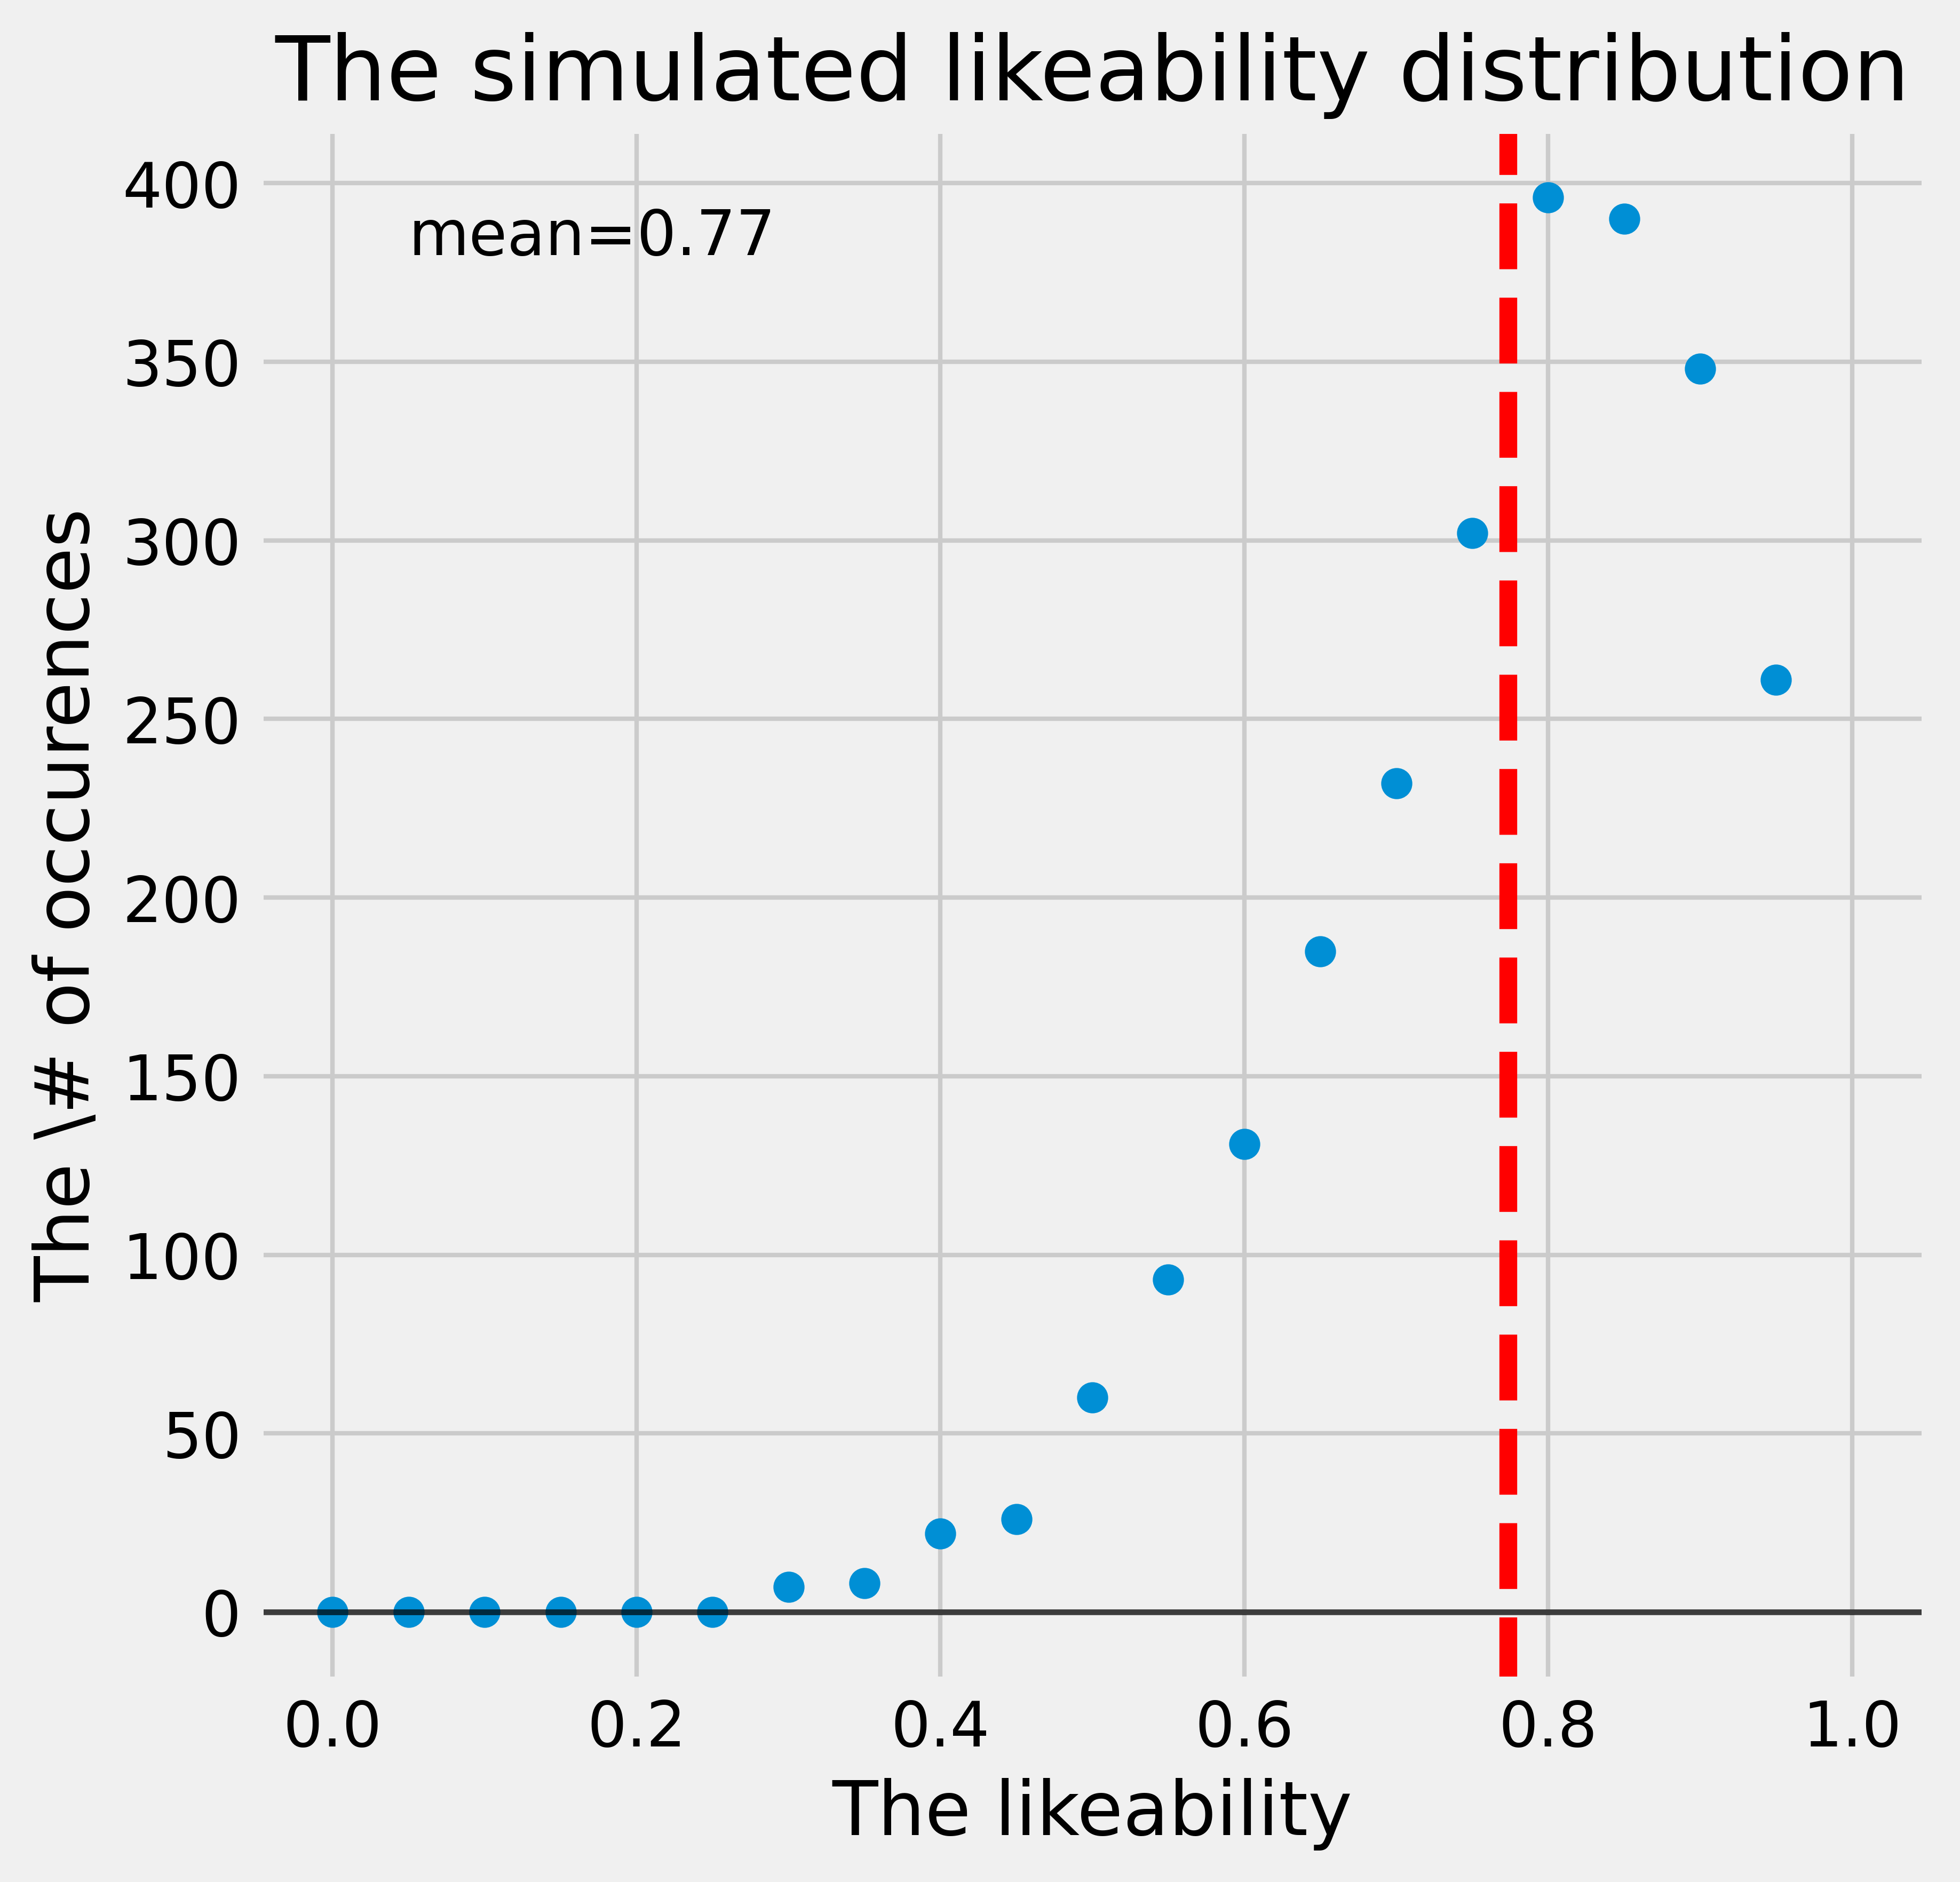
\includegraphics[width=0.42\textwidth,right]{assets/sim_ratings_v1.png}
    \caption{}
    \label{fig:sim_ratings_v1}
\end{wrapfigure}

To see the output, I ran the program with the parameters of 6 likes and 1 dislike from video one, and 1000 samples later I was greeted with the summary graph in figure \ref{fig:sim_ratings_v1}.

The blue dots in figure \ref{fig:sim_ratings_v1} represents the simulated occurence of the video ratings out of 1000 samples of a chosen likeability (the likeabilities are selected with steps of 0.05 for clarity). The red vertical line graphs the mean likeability.

The graph was both an expected and unexpected turnout. The simulation placed the likeability of video at 0.77, this is expected for there are certainly very little information available in only 7 ratings, but unexpected in size of the difference ($0.857-0.77=0.087$) against the naive likeability of 0.857. This shows that the naive likeability greatly overvalued the true likeability of the video.

\begin{wrapfigure}{r}{0.47\textwidth}
    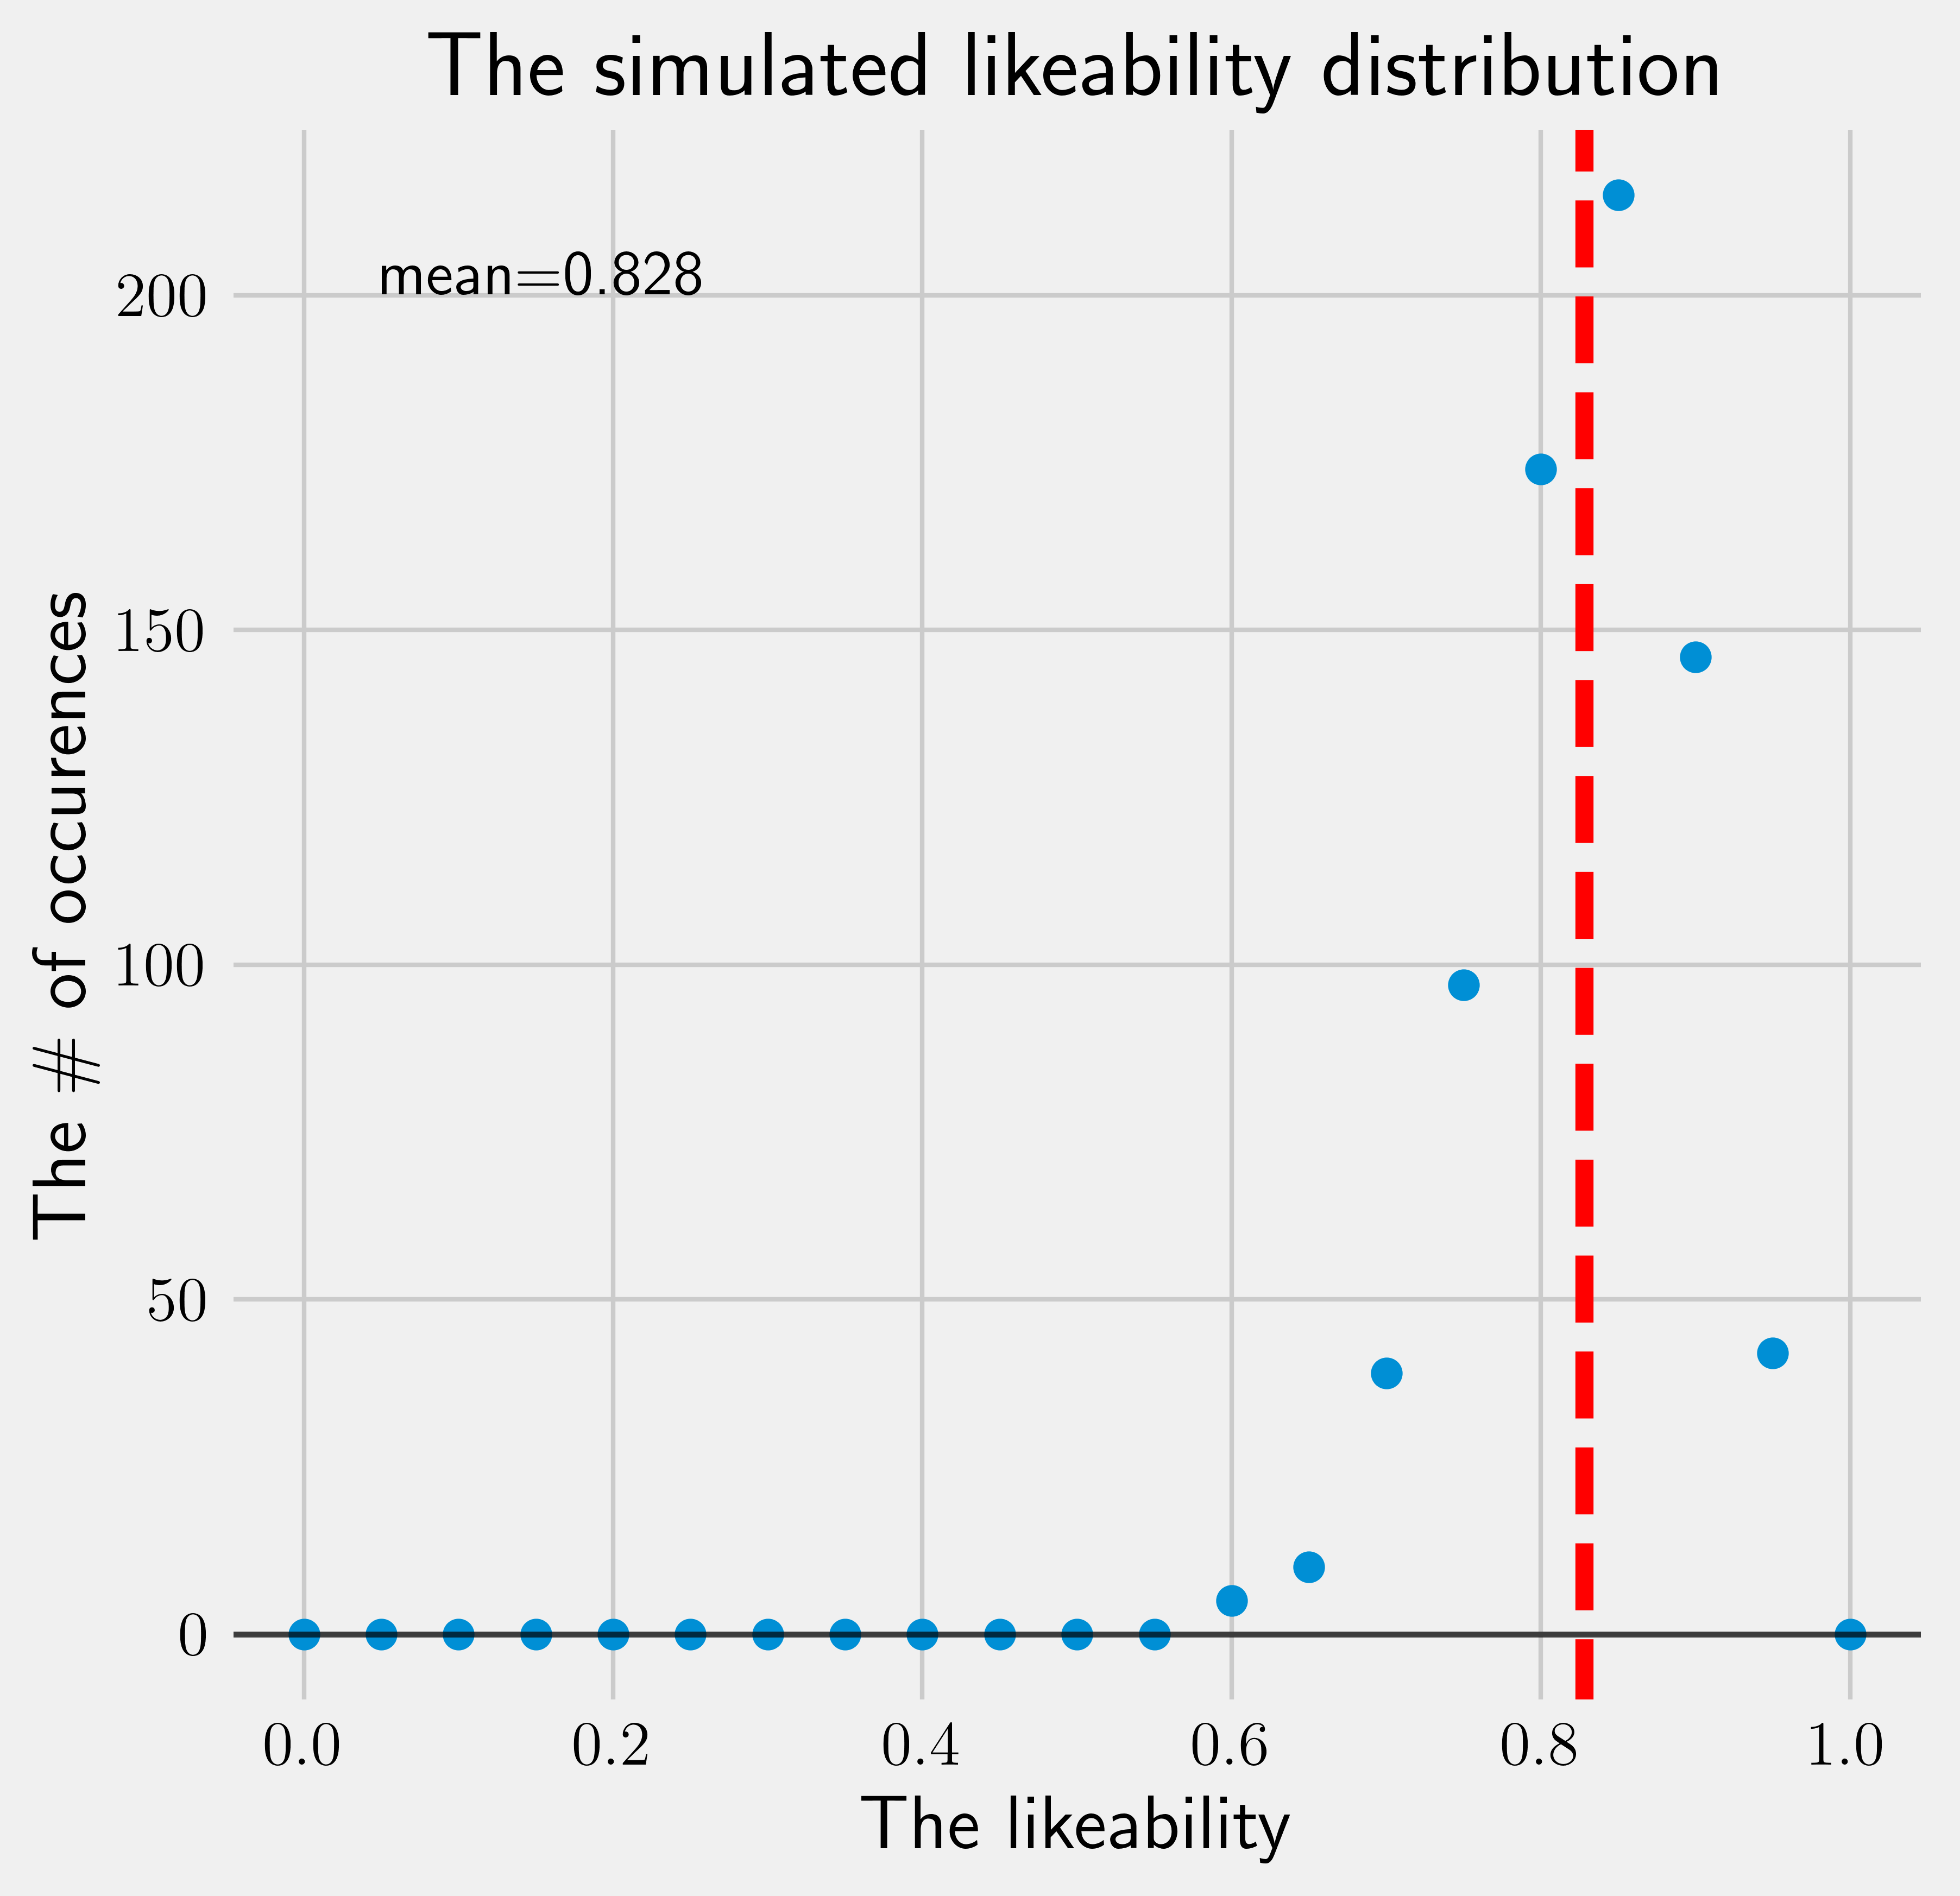
\includegraphics[width=0.42\textwidth,right]{assets/sim_ratings_v2.png}
    \caption{}
    \label{fig:sim_ratings_v2}
\end{wrapfigure}


By running the program with the parameters of the second video with 23 likes and 4 dislikes,
we obtain a mean of 0.83 and figure \ref{fig:sim_ratings_v2}.

In comparison with its naive likeability, video two is less affected by the lack of information for the simulated likeability has much smaller difference ($0.851-0.83=0.021$) than we've seen in video one. This maybe imply (appendix table) that the naive likeability increases in accuracy the more information we have, which presents an extra requirement for our analytic solution later on.

The shape of the graphs, or more formally, distributions of the likeabilities are also worth noting. They very much resemble a hill shaped curve that has a peek at only one likeability, and slopes increasing shallower the further away from the peek. Interestingly, the chosen metric of the statistical mean does not reflect the peek of the curve --- the red line does not intersect at the top of the curve. I believe this has to do with the long tail of zero occurrences at lower likeabilities, for they decreases the statistical mean in calculations.

% conclusion
Therefore the simulation approach had prove to be helpful in framing the question in finding the so called statistical mean of the range of possible likeabilities, and on top of that, had created a numerical approach of estimating the likeability of videos. But it does come at a cost of accuracy and computational time, making the method unreliable and expensive to scale up to higher amounts of ratings. Table \ref{tbl:simulation} lists the five videos and their simulated likeability values with a sample size of 1000, and step 0.01.

\begin{figure}[H]
    \centering
    \begin{tabular}{c|c|c|c|c|c}
        & Video A & Video B & Video C & Video D & Video E \\
        \hline
        \hline
        Simulated Likeability & 0.828 & 0.958 &  0.853 & 0.937 & 0.987
    \end{tabular}
    \captionof{table}{}
    \label{tbl:simulation}
\end{figure}

\section{Statistical}

% what are distributions
To search for a analytic (of symbols and operations) equation of the likeability metric, we must expand the idea of distributions that was touched on during simulations.

% examples of distributions

% the binominal

% blah

\section{Bayesian}

\section{Conclusion}

% bib


\end{document}
